\documentclass[a4paper, 12pt, twocolumn]{article} 
\setlength{\columnsep}{5mm}
\usepackage[left=1cm, top=2cm, bottom = 2cm, right=1cm, nohead, nofoot]{geometry}
\usepackage{amsthm}
\usepackage{amsmath}
\usepackage{amssymb} 
\usepackage[fleqn]{mathtools}
\usepackage{xcolor}
\definecolor{umblue}{HTML}{00274C}
\definecolor{ummaize}{HTML}{FFCB05}
\usepackage{graphicx} 
\usepackage{url}			       
\usepackage{hyperref}
\usepackage{pgf}
\usepackage{tikz}
\usetikzlibrary{arrows,automata}

\pagestyle{empty} %

\date{\today} %

\def\keywords#1{\begin{center}{\bf Keywords}\\{#1}\end{center}} %

% Please, do not change any of the above lines

\tolerance=1
\emergencystretch=\maxdimen
\hyphenpenalty=10000
\hbadness=10000

\newcommand{\XB}{\color{black}}
\newcommand{\XBB}{\color{blue}}
\newcommand{\XV}{\color{violet}}
\newcommand{\XR}{\color{red}}

\newcommand{\ds}{\displaystyle}

\begin{document}

% Type down your paper title
\title{MTH 402 CAPSTONE \\ COMMUNITY DETECTION IN NETWORKS}

\vspace{0.25cm}
% Authors
\author{Cason Konzer  \\ %
       University of Michigan - Flint \\ % Affiliation 1
       % Add authors and affiliation as needed 
       \textit{ \color{violet}
       \href{mailto:casonk@umich.edu}{casonk@umich.edu}}  % Only one corresponding e-mail
       }%

\twocolumn[
\begin{@twocolumnfalse}

\maketitle

\thispagestyle{empty}

% The abstract


\begin{abstract}

Network analysis is a growing field of study in Mathematics, Computer and Data Science. 
In the past decades many advances have been made in algorithm development and computational power. 
Applications of network analysis spread wide across many fields, some interesting examples include supply chain, social media, author citation and web page networks. 
In the this paper we start by reviewing motivations for community detection in networks, and what defines well selected communities.
To do so we discuss papers in theory, and in application, while supplementing network basics required. 
We conclude by reviewing the development of community detection algorithms, and an in depth view of select a few. 

\end{abstract}

\keywords{Communities, Networks, Social Media} % Write down at least 3 Keywords

\end{@twocolumnfalse}
]

\section{Introduction}

Within mathematics, there are certain esteemed historical problems widely taught and know by those studying the field. 
To reminisce for a moment, I was introduced to two of these problems in my discrete mathematics class while in my second semester of undergraduate education. 
The seven bridges of Königsberg and the travelling salesman problem, both problems are prominent in graph theory.
Both of these problems can be easily visualized, land masses connected by bridges and cities by roads, map reading is instilled within common human culture. 
In a similar manner a graph represented by nodes connected by edges is intuitive while scale is small. 
We can represent so much in this format, infrastructure, relationships, information flow, etc. 
Once networks become large, visualization and intuition fall off, and abstracts allow for greater understanding. 

In a brief overview of the study of networks \cite{struc_funct_cnets}, Newman focuses on real world network types, properties of networks, null graph models and processes taking place on networks. 
The study of networks in general, has drawn initial attention by mathematicians, but in the recent century, and moreover the recent decades, computer and data scientists alike have been having a field day with their applications. 
Within the even more recent years, the study of (social) media networks has grown rapidly. 
Individuals are being persuaded by bots, Trump is banned from twitter while president, and idealogies are becoming seemingly more radicalized.
Community detection and clustering is an interesting approach to tackle these issues, what if we could identify bot nets, or predict attacks by leveraging media networks?

In 2008 the Louvain algorithm \cite{louvain} for detecting communities within networks was published, and has become increasingly popular due to its advantageous run time. 
Additionally, the algorithm was shortly after extended to directed networks, akin to many media networks, and to include a `resolution' parameter \cite{louvain_resolution, com_struct_indir} providing the ability to tune for community size/density. 
Lesser known, Clauset, Newman, and Moore laid the underlying mathematics in 2004 \cite{finding_comm_struct}, Newman then extended this to weighted networks soon after \cite{analysis_of_wnets}. 
Additional community detections methods have emerged since, for example the Leiden \cite{louvain_2_leiden} and BigCLAM \cite{bigclam} algorithms. 
What is common among many of these algorithms is their way of scoring the goodness of community partitions. 
In 2003 Newman proposed the metric so called modularity leveraging the number of inter-community edges in comparison to the expectation \cite{finding_and_evaling_comm_struct}.
No matter the method, detecting communities is only an initial step to any research effort in media networks. 
To be of relevance, communities must be labeled in a meaningful way, and further their characteristics must be reviewed. 

This type of study has been of persistent interest within the social sciences. 
In the late 80s Krackhardt and Stern \cite{inet_crises} leveraged their university positions to study group dynamics of organizations via student assignments. 
A brief summary of their results finds that organizations which extend their reach externally performed superiorly. 
The so called `EI-Index' was developed as a key metric measuring the relationship between internal and external links. 
`Echochambers' and `Filter Bubbles' have become common words within the literature, and studies on media networks such as Twitter, Facebook, and Reddit \cite{eko_weko, sm_ece, ekoin_ekobtwin} are now commonplace. 
The effects of community structure and internet use in general has sparked similar research in sociology \cite{antisocial, eko_and_episteme, conspiracies_online, captivating}, and become of an increased political interest with rising concerns of impacts on today's youth. 
A thorough understanding of the structure of networks, community detection algorithms, and community analysis make for a optimistic outlook on solving societal problems stemming from media networks.

\section{Network Basics}

For ease of future discussion, let us set now some nomenclature and consider some of the first key features of networks. 
Common within literature there are two ways to refer to each of the two main ingredients of a network. 
Nodes, or vertices, are the crucial element of networks. 
Within the World Wide Web these would be web pages, within food webs these would be species, and within transit networks these may be thought of as intersections. 
On the other hand we have edges, or links, which are the glue holding nodes together and explaining their interaction. 
Within the World Wide Web these are hyperlinks, or pointers from webpage to webpage, within food webs these are these represent the predator prey relationship, and within transit networks these are the roads themselves. 

Following standard, we denote $ n $ to be the number of nodes in the network, and $ m $ the number of edges. 
Similarly, we will denote $ k_i $ as the degree of node $ i $. 
Edges can be mutual, or undirected, such that an edge between node $ i $ and $ j $ is just that. 
Also edges can be weighted, one may think of weighted edges in the example of food webs as the proportion of a species diet, or within roads as the number of lanes. 
Last edges can be directed, for example a web-link from page $ i $ to page $ j $, or a one-way street. 
In the study of real world networks, one will find common all of these edge attributes within a single graph. 

It is useful now to introduce the configuration model, of which is described in depth by Newman in \cite{networks}. 
Under this model each node has a know degree, as is often the case in network data set. 
The degree of a node is equal to the number of edges incident on it. 
As each edge is incident upon two nodes, it follows closely that summing degree across all nodes should be twice that the number of edges within the network : $ \sum_{i}^{n} k_{i} = 2m $.
For here a useful visualization is provided in Figure ~\ref{fig:spokes}, such that we view each node as depicted with spokes representing their edge connections. 
For the remainder of this paper we will denote $ s $ as the number of spokes, or twice the number of edges, within a network. 

\vspace{10mm}

\begin{figure}[h]
       \centering
       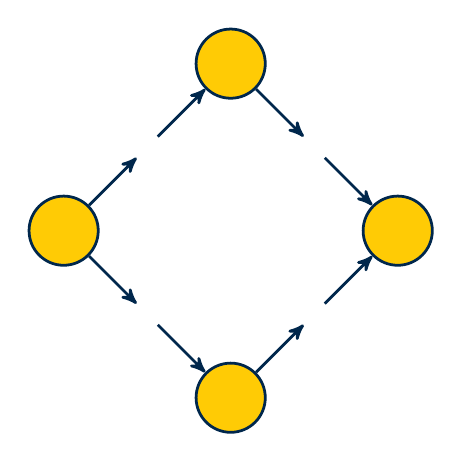
\begin{tikzpicture}[->,>=stealth',auto,node distance=1.5cm,semithick,line width=1pt]
              \tikzstyle{every state}=[fill=ummaize,draw=umblue,text=white]
              \tikzstyle{mid}=[fill=white,draw=none,text=white]
              \tikzstyle{e}=[color=umblue]
              
              \node[state]         (A)                     {};
              \node[mid]          (AB)  [above right of=A] {};
              \node[state]         (B) [above right of=AB] {};
              \node[mid]          (AC)  [below right of=A] {};
              \node[state]         (C) [below right of=AC] {};
              \node[mid]          (BD)  [below right of=B] {};
              \node[state]         (D) [below right of=BD] {};
              \node[mid]          (CD)   [below left of=D] {};
              \node[mid]          (AD)         [left of=D] {};
              
              \path  (A)  edge[e]              node {} (AB)
                     (AB) edge[e]              node {} (B)
                     (A)  edge[e]              node {} (AC)
                     (AC) edge[e]              node {} (C)
                     (B)  edge[e]              node {} (BD)
                     (BD) edge[e]              node {} (D)
                     (C)  edge[e]              node {} (CD)
                     (CD) edge[e]              node {} (D);
              
       \end{tikzpicture}
       \caption{Spoke Representation}
       \label{fig:spokes}
\end{figure}    

\newpage

\begin{figure}[t]
       \centering
       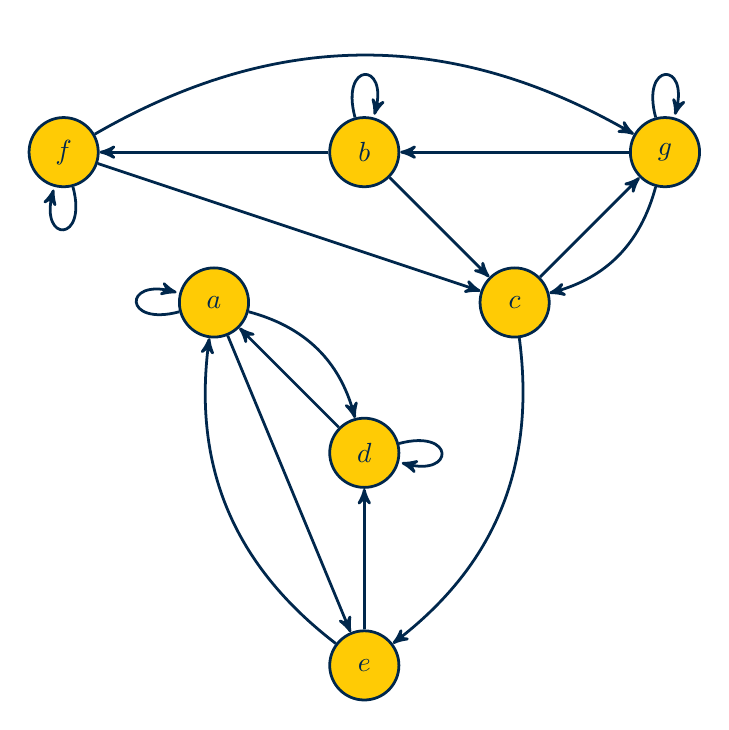
\begin{tikzpicture}[->,>=stealth',auto,node distance=2.7cm,semithick,line width=1pt]
              \tikzstyle{every state}=[fill=ummaize,draw=umblue,text=umblue]
              \tikzstyle{e}=[color=umblue]
              
              \node[state]         (A)                    {$a$};
              \node[state]         (B) [above right of=A] {$b$};
              \node[state]         (D) [below right of=A] {$d$};
              \node[state]         (C) [below right of=B] {$c$};
              \node[state]         (F) [above  left of=A] {$f$};
              \node[state]         (G) [above right of=C] {$g$};
              \node[state]         (E) [below of=D]       {$e$};
            
              \path (A) edge [e,loop  left] node {} (A)
                        edge [e]            node {} (E)
                        edge [e, bend left] node {} (D)
                    (F) edge [e,bend  left] node {} (G)
                        edge [e,loop below] node {} (F)
                        edge [e]            node {} (C)
                    (B) edge [e,loop above] node {} (B)
                        edge [e]            node {} (C)
                        edge [e]            node {} (F)
                    (G) edge [e]            node {} (B)
                        edge [e,loop above] node {} (G)
                        edge [e,bend  left] node {} (C)
                    (C) edge [e]            node {} (G)
                        edge [e,bend  left] node {} (E)
                    (D) edge [e,loop right] node {} (D)
                        edge [e]            node {} (A)
                    (E) edge [e,bend  left] node {} (A)
                        edge [e]            node {} (D);
              
       \end{tikzpicture}
       \caption{Example Network}
       \label{fig:ex_network}
\end{figure}    


A standard representation of networks is via an adjacency matrix, denoted $ A $. 
The entry $ A_{i,j} $ represents the number of edges from node $ i $ to node $ j $. 
A practical way to represent weighted networks is let the weights represent the number of edges, in the case of non-integer weights, a simple scaling can be applied to transform the matrix into one with integer only entries. 
In undirected networks, adjacency matrices exhibit symmetry across the diagonal. 
For the given network in Figure ~\ref{fig:ex_network}, we see the following directed adjacency matrix :

% \vspace{1mm}

\begin{center}
       \begin{tabular}{c|ccccccc} 
              $ A $ & $ a $ & $ b $ & $ c $ & $ d $ & $ e $ & $ f $ & $ g $ \\
              \hline
              $ a $ & $ 1 $ & $ 0 $ & $ 0 $ & $ 1 $ & $ 1 $ & $ 0 $ & $ 0 $ \\
              $ b $ & $ 0 $ & $ 1 $ & $ 1 $ & $ 0 $ & $ 0 $ & $ 1 $ & $ 0 $ \\
              $ c $ & $ 0 $ & $ 0 $ & $ 0 $ & $ 0 $ & $ 1 $ & $ 0 $ & $ 1 $ \\
              $ d $ & $ 1 $ & $ 0 $ & $ 0 $ & $ 1 $ & $ 0 $ & $ 0 $ & $ 0 $ \\
              $ e $ & $ 1 $ & $ 0 $ & $ 0 $ & $ 1 $ & $ 0 $ & $ 0 $ & $ 0 $ \\
              $ f $ & $ 0 $ & $ 0 $ & $ 1 $ & $ 0 $ & $ 0 $ & $ 1 $ & $ 1 $ \\
              $ g $ & $ 0 $ & $ 1 $ & $ 1 $ & $ 0 $ & $ 0 $ & $ 0 $ & $ 1 $ \\
       \end{tabular}
\end{center}

% \vspace{1mm}

\noindent
Similarly if we consider Figure ~\ref{fig:ex_network} as an undirected graph, we have the adjacency matrix :

% \vspace{1mm}

\begin{center}
       \begin{tabular}{c|ccccccc} 
              $ A $ & $ a $ & $ b $ & $ c $ & $ d $ & $ e $ & $ f $ & $ g $ \\
              \hline
              $ a $ & $ 1 $ & $ 0 $ & $ 0 $ & $ 2 $ & $ 1 $ & $ 0 $ & $ 0 $ \\
              $ b $ & $ 0 $ & $ 1 $ & $ 1 $ & $ 0 $ & $ 0 $ & $ 1 $ & $ 1 $ \\
              $ c $ & $ 0 $ & $ 1 $ & $ 0 $ & $ 0 $ & $ 1 $ & $ 1 $ & $ 2 $ \\
              $ d $ & $ 2 $ & $ 0 $ & $ 0 $ & $ 1 $ & $ 1 $ & $ 0 $ & $ 0 $ \\
              $ e $ & $ 1 $ & $ 0 $ & $ 1 $ & $ 1 $ & $ 0 $ & $ 0 $ & $ 0 $ \\
              $ f $ & $ 0 $ & $ 1 $ & $ 1 $ & $ 0 $ & $ 0 $ & $ 1 $ & $ 1 $ \\
              $ g $ & $ 0 $ & $ 1 $ & $ 2 $ & $ 0 $ & $ 0 $ & $ 1 $ & $ 1 $ \\
       \end{tabular}
\end{center}

\section{Good Communities}

With the fundamentals of networks we can now dive into the underlying mechanics of many community detection algorithms, modularity. 
One underlying assumption of judging community fit is that the information to perform such judgment is provided within the network itself \cite{network_science}. 
Of course in some real world networks the information may be available explicitly, such as groups formed on social media platforms. 
With this said such additional information can be used to baseline the metric here forward defined \cite{finding_and_evaling_comm_struct}.
The form in which communities exist imposes an additional constraint, in that we will require communities to be disjoint. 
Of course this is again not always the case, as nodes may exist embedded in multiple communities. 

The next assumption for good communities is that they have a proportionally higher number of internal links compared to that of external links. 
As the sum of these two proportions encompasses all of the links attached to nodes within a community it is sufficient to consider only one of the two figures. 
Good communities would then either have a maximized number of internal links, or otherwise a minimized number of external links. 
To clarify to the reader, internal links are edges connected to nodes of which both exist within the community. 
External links consist of strictly one node within the community, and edges connecting two nodes outside a community are disregarded for the figure. 
Following, it is such that analysis is conducted on a per community basis, and the goodness of the graph partition is evaluated as a sum of modularity values across all communities within the graph. 
With these assumption there is one issue persistent, always, the trivial case where the whole graph itself is selected as one giant community, would maximize modularity as outlined above \cite{finding_comm_struct}. 

To improve modularity such that it is a useful measure, we may consider the expectation of internal and external links as well. 
If we find that the communities detected within a graph have a higher number of internal links than the expected number of internal links, we are able to mitigate the issue with finding giant communities. 
In addition, it is often a question as to how many communities an algorithm should be tuned to find, under the modularity maximization approach the number is discovered and corresponds to the number of communities found when modularity is at it's maximum. 

Let us now examine the expected number internal edges. 
For initial analysis, let us consider the undirected network case. 
One piece of information we know is the degree of each node, and thus can leveraged analysis from the configuration model. 
Let us first consider the expected number of edges between any two nodes, denoted $ \mathbb{E}(i, j) $ for given nodes $ i $ and $ j $. 
For two distinct nodes, we have $ k_{i}k_{j} $ ways to connected the spokes between them. 
For any one spoke, there exists $ s - 1 $ other spokes to which it can connect, as a spoke cannot connect to itself. 
It follows that the probability one spoke connects with any other spoke is $ \frac{1}{s - 1} $.  
Summing of all possibly ways to connect two distinct nodes, we find then $ \mathbb{E}(i, j) = \frac{k_{i}k_{j}}{s - 1} $. 
In the case that the nodes are not distinct, e.g. the case for self loops, the node has $ k_{i} $ spokes, each of which could connect to $ k_{i} - 1 $ other spokes attached to the same node. 
The the expected number of self edges for a given node is $ \mathbb{E}(i, i) = \frac{k_{i}(k_{i} - 1)}{s - 1} $.
A quick check summing over all node pairs, should yield the total number of spokes, as each edge is connected to two nodes. 

\begin{flalign*}
       & \ds \sum_{i, j}^{n} \mathbb{E}(i, j) = \sum_{i, j \ne i}^{n} \mathbb{E}(i, j) + \sum_{i}^{n} \mathbb{E}(i, i) \\
       &= \sum_{i, j \ne i}^{n} \frac{k_{i}k_{j}}{s - 1} + \sum_{i}^{n} \frac{k_{i}(k_{i} - 1)}{s - 1} \\
       &= \frac{1}{s - 1} \left[ \sum_{i}^{n} k_{i} \sum_{j \ne i}^{n} k_{j} + \sum_{i}^{n} k_{i} \sum_{i}^{n} k_{i} - \sum_{i}^{n} k_{i} \right] \\
       &= \frac{1}{s - 1} \left[ \sum_{i}^{n} k_{i} \sum_{j}^{n} k_{j} - s \right] \\
       &= \frac{s^{2} - s}{s - 1} = \frac{s(s - 1)}{s - 1} = s
\end{flalign*}

Knowing now the expected number of edges between two nodes, let us consider all nodes in a community, for all communities within the graph. 
Modularity is represent forward as the normalized value $ Q = C_{\% \ internal} - C_{\% \ \mathbb{E} \ internal} $. 
Here $ C_{\% \ internal} $ is the percentage of the internal community links within the graph and $ C_{\% \ \mathbb{E} \ internal} $ is the expected percentage of the internal community links within the graph respectively.
The metric bounded by $ -1 $ and $ 1 $, in the case where our found internal links math exactly that of the expected number by random linking of nodes, we find $ Q = 0 $, which now corresponds to the trivial case where we find one giant community. 

To formalize this method it is easiest to think in terms of spokes rather than edges. 
Letting $ c_{i} $ represent the community in which node $ i $ belongs, we can create an indicator function $ \delta(c_{i}, c_{j}) $ evaluating to $ 1 $ given nodes $ i $ and $ j $ are in the same community, and $ 0 $ otherwise. 
This provides an easy way to now identify the true percentage of internal community link found within the graph after detected. 

\begin{flalign*}
       & \ds C_{\% \ internal} = \frac{1}{s} \left[ \sum_{i, j}^{n} A_{i, j} \delta(c_{i}, c_{j}) \right] 
\end{flalign*}

\noindent
The indicator function additionally provides an easy way to calculate the expected percentage of internal links. 

\begin{flalign*}
       & \ds C_{\% \ \mathbb{E} \ internal} = \frac{1}{s} \left[ \sum_{i, j \ne i}^{n} \frac{k_{i}k_{j}}{s - 1} \delta(c_{i}, c_{j}) + \sum_{i}^{n} \frac{k_{i}(k_{i} - 1)}{s - 1}\right] 
\end{flalign*}

\noindent
Form here we can now formalize modularity. 

\begin{multline*}
       \ds Q = \frac{1}{s} \Biggl[ \sum_{i, j \ne i}^{n} \left( A_{i, j} - \frac{k_{i}k_{j}}{s - 1} \right) \delta(c_{i}, c_{j}) \\ 
       +  \sum_{i}^{n} \left( A_{i,i} - \frac{k_{i}(k_{i} - 1)}{s - 1} \right) \Biggr] 
\end{multline*}

The traditional formulation of modularity makes two additional simplifications based on large scale real world networks. 
First, as networks grow large the subtraction of $ 1 $ from the number of possible spoke to spoke connections becomes negligible. 
Formally, $ \lim_{s \rightarrow \infty} \frac{k_{i}k_{j}}{s - 1} = \frac{k_{i}k_{j}}{s} $.
Second, the number of self edges is proportionally small compared to the total number of edges, and can be treated as if the repeated nodes are distinct. 
Applying these two heuristics we come to the traditional definition of modularity. 

\begin{flalign*}
       & \ds Q = \frac{1}{s} \Biggl[ \sum_{i, j}^{n} \left( A_{i, j} - \frac{k_{i}k_{j}}{s} \right) \delta(c_{i}, c_{j})  \Biggr] 
\end{flalign*}

\noindent
The definition calculates the modularity for the graph in whole by leveraging our indicator function.
After detecting communities a simple evaluation of $ Q $ can quantify the goodness of the graph's partition. 

Without any alteration to the definition, the definition holds for weighted graphs given the perspective shift form edge weightings to edge counts achieved by converting a weighted graph to a multigraph \cite{analysis_of_wnets}. 
With a few adjustments, we can extend our definition to directed graphs as well \cite{com_struct_indir}. 
First we must notice that each node has two degree types, indegree and outdegree, denoted $ k_{i}^{in} $ and $ k_{i}^{out} $ respectively for node $ i $.
We now have two equations $ \sum_{i}^{n} k_{i}^{in} = m $ and $ \sum_{i}^{n} k_{i}^{out} = m $, such that $ \sum_{i}^{n} \left( k_{i}^{in} + k_{i}^{out} \right) = s $.
As we now count edges only once in our adjacency matrix, we divide our summation by $ m $ rather than $ s $.
Similarly in our expectation, the probability of an outward spoke connecting to any inward spoke becomes $ \frac{1}{m} $. 
Within this case it is no longer necessary for the subtraction of the initial spoke as it is not one of the total inward spokes. 
Thus summing over all possibly ways to have a edges going from node $ i $ to node $ j $ is $ \frac{k_{i}^{in}k_{j}^{out}}{m} $. 
It follows nicely that our directed modularity $ Q_{dir} $ is similarly defined. 

\begin{flalign*}
       & \ds Q_{dir} = \frac{1}{m} \Biggl[ \sum_{i, j}^{n} \left( A_{i, j} - \frac{k_{i}^{in}k_{j}^{out}}{m} \right) \delta(c_{i}, c_{j}) \Biggr] 
\end{flalign*}

We now have the ability to judge graph community partition and additionally have a metric on which we wish to optimize within community detection algorithms. 
From experimental data, it is accepted that a modularity value greater than or equal to $ 0.3 $ represents significant community structure \cite{finding_comm_struct}. 

For an illustrative example consider Figure ~\ref{fig:ex_comms}, given the selected communities identified by node color. 
We have the prior directed adjacency matric, and the following expectation matrix : 

\begin{center}
       \begin{tabular}{c|ccccccc} 
              $ \mathbb{E} $ & $ a $ & $ b $ & $ c $ & $ d $ & $ e $ & $ f $ & $ g $ \\
              \hline
              $ a $ & $ \frac{9}{15} $ & $ \frac{9}{15} $ & $ \frac{3}{15} $ & $ \frac{6}{15} $ & $ \frac{6}{15} $ & $ \frac{9}{15} $ & $ \frac{9}{15} $ \\
              $ b $ & $ \frac{6}{15} $ & $ \frac{6}{15} $ & $ \frac{2}{15} $ & $ \frac{4}{15} $ & $ \frac{4}{15} $ & $ \frac{6}{15} $ & $ \frac{9}{15} $ \\
              $ c $ & $ \frac{9}{15} $ & $ \frac{9}{15} $ & $ \frac{3}{15} $ & $ \frac{6}{15} $ & $ \frac{6}{15} $ & $ \frac{9}{15} $ & $ \frac{9}{15} $ \\
              $ d $ & $ \frac{9}{15} $ & $ \frac{9}{15} $ & $ \frac{3}{15} $ & $ \frac{6}{15} $ & $ \frac{6}{15} $ & $ \frac{9}{15} $ & $ \frac{9}{15} $ \\
              $ e $ & $ \frac{6}{15} $ & $ \frac{6}{15} $ & $ \frac{2}{15} $ & $ \frac{4}{15} $ & $ \frac{4}{15} $ & $ \frac{6}{15} $ & $ \frac{6}{15} $ \\
              $ f $ & $ \frac{6}{15} $ & $ \frac{6}{15} $ & $ \frac{2}{15} $ & $ \frac{4}{15} $ & $ \frac{4}{15} $ & $ \frac{6}{15} $ & $ \frac{6}{15} $ \\
              $ g $ & $ \frac{9}{15} $ & $ \frac{9}{15} $ & $ \frac{3}{15} $ & $ \frac{6}{15} $ & $ \frac{6}{15} $ & $ \frac{9}{15} $ & $ \frac{9}{15} $ \\
       \end{tabular}
\end{center}

similarly $ A_{i, j} - \frac{k_{i}^{in}k_{j}^{out}}{m} $ becomes :

\begin{center}
       \begin{tabular}{c|ccccccc} 
              $ A_{i, j} - \mathbb{E} $ & $ a $ & $ b $ & $ c $ & $ d $ & $ e $ & $ f $ & $ g $ \\
              \hline
              $ a $ & $ \frac{6}{15}  $ & $ \frac{-9}{15} $ & $ \frac{-3}{15} $ & $ \frac{9}{15}  $ & $ \frac{9}{15}  $ & $ \frac{-9}{15} $ & $ \frac{-9}{15} $ \\
              $ b $ & $ \frac{-6}{15} $ & $ \frac{9}{15}  $ & $ \frac{13}{15} $ & $ \frac{-4}{15} $ & $ \frac{-4}{15} $ & $ \frac{9}{15}  $ & $ \frac{-9}{15} $ \\
              $ c $ & $ \frac{-9}{15} $ & $ \frac{-9}{15} $ & $ \frac{-3}{15} $ & $ \frac{-6}{15} $ & $ \frac{9}{15}  $ & $ \frac{-9}{15} $ & $ \frac{6}{15}  $ \\
              $ d $ & $ \frac{6}{15}  $ & $ \frac{-9}{15} $ & $ \frac{-3}{15} $ & $ \frac{9}{15}  $ & $ \frac{-6}{15} $ & $ \frac{-9}{15} $ & $ \frac{-9}{15} $ \\
              $ e $ & $ \frac{9}{15}  $ & $ \frac{-6}{15} $ & $ \frac{-2}{15} $ & $ \frac{11}{15} $ & $ \frac{-4}{15} $ & $ \frac{-6}{15} $ & $ \frac{-6}{15} $ \\
              $ f $ & $ \frac{-6}{15} $ & $ \frac{-6}{15} $ & $ \frac{13}{15} $ & $ \frac{-4}{15} $ & $ \frac{-4}{15} $ & $ \frac{9}{15}  $ & $ \frac{9}{15}  $ \\
              $ g $ & $ \frac{-9}{15} $ & $ \frac{6}{15}  $ & $ \frac{12}{15} $ & $ \frac{-6}{15} $ & $ \frac{-6}{15} $ & $ \frac{-9}{15} $ & $ \frac{6}{15}  $ \\
       \end{tabular}
\end{center}

$ \delta(c_{i}, c_{j}) $ is :

\begin{center}
       \begin{tabular}{c|ccccccc} 
              $ \delta(c_{i}, c_{j}) $ & $ a $ & $ b $ & $ c $ & $ d $ & $ e $ & $ f $ & $ g $ \\
              \hline
              $ a $ & $ 1 $ & $ 0 $ & $ 0 $ & $ 1 $ & $ 1 $ & $ 0 $ & $ 0 $ \\
              $ b $ & $ 0 $ & $ 1 $ & $ 1 $ & $ 0 $ & $ 0 $ & $ 1 $ & $ 1 $ \\
              $ c $ & $ 0 $ & $ 1 $ & $ 1 $ & $ 0 $ & $ 0 $ & $ 1 $ & $ 1 $ \\
              $ d $ & $ 1 $ & $ 0 $ & $ 0 $ & $ 1 $ & $ 1 $ & $ 0 $ & $ 0 $ \\
              $ e $ & $ 1 $ & $ 0 $ & $ 0 $ & $ 1 $ & $ 1 $ & $ 0 $ & $ 0 $ \\
              $ f $ & $ 0 $ & $ 1 $ & $ 1 $ & $ 0 $ & $ 0 $ & $ 1 $ & $ 1 $ \\
              $ g $ & $ 0 $ & $ 1 $ & $ 1 $ & $ 0 $ & $ 0 $ & $ 1 $ & $ 1 $ \\
       \end{tabular}
\end{center}

\begin{figure}[t]
       \centering
       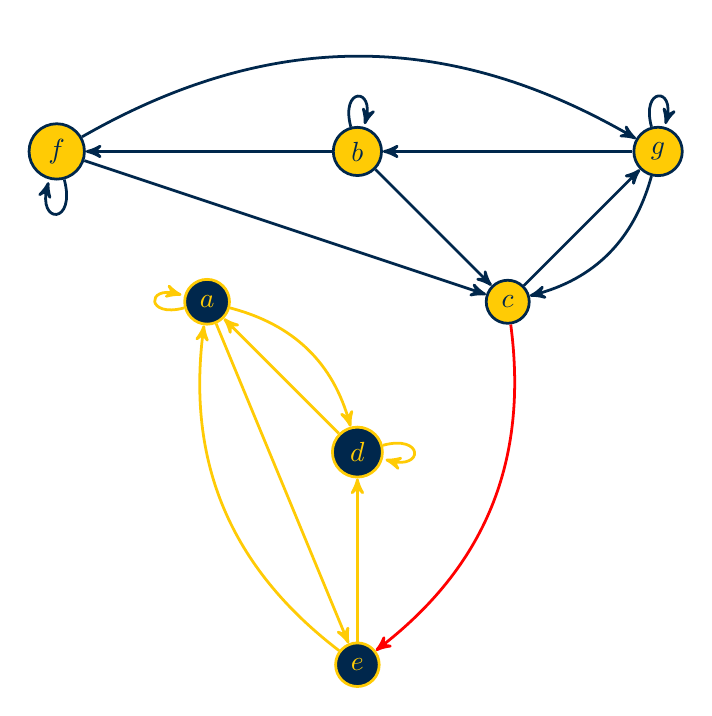
\begin{tikzpicture}[->,>=stealth',node distance=2.7cm,semithick,line width=1pt]
              \tikzstyle{dstate}=[circle,fill=ummaize,draw=umblue,text=umblue,scale=1]
              \tikzstyle{cstate}=[circle,fill=umblue,draw=ummaize,text=ummaize,scale=1]
              \tikzstyle{be}=[color=umblue]
              \tikzstyle{me}=[color=ummaize]
              \tikzstyle{re}=[color=red]
              
              \node[cstate]        (A)                    {$a$};
              \node[dstate]        (B) [above right of=A] {$b$};
              \node[cstate]        (D) [below right of=A] {$d$};
              \node[dstate]        (C) [below right of=B] {$c$};
              \node[dstate]        (F) [above  left of=A] {$f$};
              \node[dstate]        (G) [above right of=C] {$g$};
              \node[cstate]        (E) [below of=D]       {$e$};
            
              \path (A) edge [me,loop  left] node {} (A)
                        edge [me]            node {} (E)
                        edge [me, bend left] node {} (D)
              (F) edge [be,bend  left] node {} (G)
                        edge [be,loop below] node {} (F)
                        edge [be]            node {} (C)
                    (B) edge [be,loop above] node {} (B)
                        edge [be]            node {} (C)
                        edge [be]            node {} (F)
                    (G) edge [be]            node {} (B)
                        edge [be,loop above] node {} (G)
                        edge [be,bend  left] node {} (C)
                    (C) edge [be]            node {} (G)
                        edge [re,bend  left] node {} (E)
                    (D) edge [me,loop right] node {} (D)
                        edge [me]            node {} (A)
                    (E) edge [me,bend  left] node {} (A)
                        edge [me]            node {} (D);
              
       \end{tikzpicture}
       \caption{Example Community Partition}
       \label{fig:ex_comms}
\end{figure}  

Last denoting $ || M || $ as the sum of all entries in the matrix $ M $, $ Q = \frac{1}{m} || (A_{i, j} - \mathbb{E}) \delta(c_{i}, c_{j}) || = 0.42 \overline{6} $.
We would thus consider that this graph exhibits strong community structure with the given partition. 
Due to the small scale of this graph it is easy to identify well a good partition, but as networks scale visualization becomes increasingly challenging, and thus such an approach as we have outlined is required for analysis. 

\section{Evolution of Algorithms}

Algorithms are most commonly judged on complexity, but there is a clear tradeoff with accuracy. 
With modularity there is a proxy metric to judge the accuracy of a community detection algorithm. 
Traditionally, accuracy is defined with a ground truth, such that the true community structure is known within the network. 
Computational complexity is a good reference for scalability of an algorithm, and the upper limit of size of useable networks. 
Additionally as time goes one, as Moore's Law realizes, a phenomena that the size of usable networks with fixed complexity increases dependent on the temporal increase in computational power. 
With that said for a given dataset, one may be able to execute a more complex algorithm with increased accuracy, in the same run time as a simpler algorithm in the same ran years prior. 
The evolution of algorithms plays on both of these characteristics. 

The first proposal of the modularity to the best of our knowledge comes from Newman in \cite{finding_and_evaling_comm_struct}. 
The application was applied to the simplest of networks, undirected and unweighted. 
Modularity was simply used to evaluate goodness of community detection, and impose a stopping condition of the detection algorithm. 
Two detection techniques were utilized, both of which unutilized edge removal based on a betweenness measure. 
The simpler of the two methods, was to calculate shortest-path betweenness. 
The second method focused on random-walk, or otherwise equivalently current-flow betweenness. 
In both cases, the assumption is that many nodes must flow thorough community-to-community edges. 
In the case of removing these community connecting edges one expects to find the underlying communities. 
In general, the algorithm would be ran until no edges exist. 
After each edge removal, the graphs modularity is calculated. 
The best partition is then selected, such that modularity is maximized.

It is noticed that there are two forms of which modularity optimization can occur. 
Modularity can be single peaked, such that there is both one global and local maxima. 
Similarly modularity can be multipeaked, such that there is one global but multiple local maxima. 
In either case, one could halt the algorithm after finding the first local maxima. 
In the multipeaked case the shall give a `good' partition but not necessarily the best, introducing a probability for reduced accuracy. 
In the single peaked case this technique provides the optimal partition. 
Clearly, this will reduce the runtime of the algorithm, and is a tradeoff considered by the implemented dependent upon the size of their network. 

Historically (pre 2000) algorithms were agglomerative (bottom up), finding communities by the addition of edges rather than removal, such as the well known k-means clustering \cite{least_squares_PCM, some_methods}. 
Newman's work shifted the state of the are to decisive (top down) algorithms \cite{com_struct_in_soc_and_bio}. 
Soon after Newman's initial work he extended his algorithm to weighted networks \cite{analysis_of_wnets}, thereafter developing an algorithm for modularity maximization with reduced complexity \cite{finding_comm_struct}.
Later work by Newman extended the algorithm to directed networks \cite{com_struct_indir} for increased accuracy, while in parallel Blondel, Guillaume, Lambiotte, and Lefebvre made significant strides in complexity reduction allowing for analysis of massive networks in the so-called Louvain algorithm \cite{louvain}. 
Continuing later the Louvain algorithm was extend to directed networkes by Dugu{\'e} and Perez to account for the additional information provided within the links \cite{directed_louvain}. 
Coming to some of the most recent developments the Louvain algorithm was transformed to the Leiden algorithm with an additional reduction in complexity by Traag, Waltman, and van Eck in 2019 \cite{louvain_2_leiden}. 

% \section{Analysis of Algorithms}

\section{Conclusion}

In this disussion we have identified basics of networks, reviewed the mechanics of disjoint community detection within network, and discussed the history of community detection algorithms. 
Future work shall include an analysis of the algorithms aforementioned, providing deeper insights into the relevance of historical advancements. 
Additional work permits review of overlapping community detection algorithms, along with their sequential development. 
Worth while is to weight the pros and cons of disjoint vs. overlapping algorithms. 
As computational power and datasets grow, an understanding of where we come from is crucial to proper implementation and selection of cutting edge network algorithms.

\bibliography{multipager.bib}{}
\bibliographystyle{plain}

% \end{multicols}
\end{document}